\chapter{Multiphysics topology optimization problems}

In this chapter we will focus on the effects of multiphysics couplings in nanophotonic devices, reviewing state-of-the-art research, 
highlighting open topology optimization problems, and presenting our contributions to the field.
We will focus on three main classes of multiphysics couplings: thermo-optical, opto-mechanical, and electro-optical systems.
%\begin{figure}[tb]
%    \centering
%    \makebox[\textwidth][c]{\includegraphics[width=1\imwidth]{figures/simpModel.png}}%
%    \caption{Bla bla bla...}
%    \label{fig:illustateTopOpt}
%\end{figure}


%\begin{equation}
%    (EIu'')'' = q
%\end{equation}


%\begin{figure}[tb]
%    \centering
%    \makebox[\textwidth][c]{\begin{tikzpicture}[remember picture]
    \begin{scope}[xshift=0mm]
        % angle (deg)
        \newcommand\ai{10}
        % line width
        \newcommand\wi{1pt}
        % cell size
        \newcommand\cellsize{3}
        % Rank-$N$ size
        \newcommand\di{0.75}

        % cell
        \draw[gray!10,   fill=gray!10, rotate around={\ai:(0,0)}] (0,0) rectangle (\cellsize,\cellsize) node (rect1) {};
        \draw[black!60, fill=black!60, rotate around={\ai:(0,0)}] (0,0) rectangle (\di,\cellsize);

        % orientation frame
        \draw[black, -stealth, line width=\wi, rotate around={\ai:({\di*cos(\ai) - \cellsize/2*sin(\ai)},{\di*sin(\ai) + \cellsize/2*cos(\ai)})}] ({\di*cos(\ai) - \cellsize/2*sin(\ai)},{\di*sin(\ai) + \cellsize/2*cos(\ai)}) -- ({\di*cos(\ai) - \cellsize/2*sin(\ai) + 0.75},{\di*sin(\ai) + \cellsize/2*cos(\ai)});
        \draw[black, -stealth, line width=\wi, rotate around={\ai:({\di*cos(\ai) - \cellsize/2*sin(\ai)},{\di*sin(\ai) + \cellsize/2*cos(\ai)})}] ({\di*cos(\ai) - \cellsize/2*sin(\ai)},{\di*sin(\ai) + \cellsize/2*cos(\ai)}) -- ({\di*cos(\ai) - \cellsize/2*sin(\ai)},{\di*sin(\ai) + \cellsize/2*cos(\ai) + 0.75});

        % local frame
        \draw[black, -stealth, dashed, line width=\wi] (0,0) -- ({\cellsize + 0.8},0);
        \draw[black, -stealth, dashed, line width=\wi] (0,0) -- (0,{\cellsize + 0.8});

        % ruler
        \draw[black, |-|, line width=\wi, rotate around={\ai:(0,0)}] (0,0) -- (\cellsize,0);
        \draw[black,  -|, line width=\wi, rotate around={\ai:(0,0)}] (0,0) -- (\di,0);

        % arc
        \draw[black, dotted, line width=\wi] (\cellsize,0) arc (0:\ai:\cellsize);

        % annotation
        \draw (\cellsize + 0.7, -0.3) node {$x_1 / \epsilon^3$};
        \draw (-0.5, \cellsize + 0.8) node {$x_2 / \epsilon^3$};
        \draw (\cellsize/2,-0.75) node {Rank-$1$};

        \draw[rotate around={{\ai/2}:(0,0)}] ({\cellsize+0.3},0) node {$\theta_1$};

        \draw[rotate around={{\ai}:(0,0)}] ({\di/2},0.4) node [rotate around={{\ai}:(0,0)}] {$\mu_1$};
        \draw[rotate around={{\ai}:(0,0)}] ({(\cellsize - \di)/2 + \di},0.4) node [rotate around={{\ai}:(0,0)}] {$1-\mu_1$};

        \draw[rotate around={{\ai}:(0,0)}] ({0+0.4},{\cellsize-0.4}) node [rotate around={{\ai}:(0,0)}] {$(+)$};
        \draw[rotate around={{\ai}:(0,0)}] ({\cellsize-0.4},{\cellsize-0.4}) node [rotate around={{\ai}:(0,0)}] {$(-)$};
        \coordinate (A) at (rect1.north);


        \draw[rotate around={\ai:({\di*cos(\ai) - \cellsize/2*sin(\ai)},{\di*sin(\ai) + \cellsize/2*cos(\ai)})}] ({\di*cos(\ai) - \cellsize/2*sin(\ai)+1} , {\di*sin(\ai) + \cellsize/2*cos(\ai) + 0.2}) node {$\mathbf{n}_1$};
        \draw[rotate around={\ai:({\di*cos(\ai) - \cellsize/2*sin(\ai)},{\di*sin(\ai) + \cellsize/2*cos(\ai)})}] ({\di*cos(\ai) - \cellsize/2*sin(\ai) + 0.3} , {\di*sin(\ai) + \cellsize/2*cos(\ai) + 1}) node {$\mathbf{m}_1$};



    \end{scope}
    \begin{scope}[xshift=45mm]
        % angle (deg)
        \newcommand\ai{15}
        % line width
        \newcommand\wi{1pt}
        % cell size
        \newcommand\cellsize{3}
        % Rank-$N$ size
        \newcommand\di{0.6}

        % cell
        \draw[gray!40,   fill=gray!40, rotate around={\ai:(0,0)}] (0,0) rectangle (\cellsize,\cellsize) node (rect2) {};
        \draw[black!60, fill=black!60, rotate around={\ai:(0,0)}] (0,0) rectangle (\di,\cellsize);

        % orientation frame
        \draw[black, -stealth, line width=\wi, rotate around={\ai:({\di*cos(\ai) - \cellsize/2*sin(\ai)},{\di*sin(\ai) + \cellsize/2*cos(\ai)})}] ({\di*cos(\ai) - \cellsize/2*sin(\ai)},{\di*sin(\ai) + \cellsize/2*cos(\ai)}) -- ({\di*cos(\ai) - \cellsize/2*sin(\ai) + 0.75},{\di*sin(\ai) + \cellsize/2*cos(\ai)});
        \draw[black, -stealth, line width=\wi, rotate around={\ai:({\di*cos(\ai) - \cellsize/2*sin(\ai)},{\di*sin(\ai) + \cellsize/2*cos(\ai)})}] ({\di*cos(\ai) - \cellsize/2*sin(\ai)},{\di*sin(\ai) + \cellsize/2*cos(\ai)}) -- ({\di*cos(\ai) - \cellsize/2*sin(\ai)},{\di*sin(\ai) + \cellsize/2*cos(\ai) + 0.75});

        % local frame
        \draw[black, -stealth, dashed, line width=\wi] (0,0) -- ({\cellsize + 0.8},0);
        \draw[black, -stealth, dashed, line width=\wi] (0,0) -- (0,{\cellsize + 0.8});

        % ruler
        \draw[black, |-|, line width=\wi, rotate around={\ai:(0,0)}] (0,0) -- (\cellsize,0);
        \draw[black,  -|, line width=\wi, rotate around={\ai:(0,0)}] (0,0) -- (\di,0);

        % arc
        \draw[black, dotted, line width=\wi] (\cellsize,0) arc (0:\ai:\cellsize);

        % annotation
        \draw (\cellsize + 0.7, -0.3) node {$x_1 / \epsilon^2$};
        \draw (-0.5, \cellsize + 0.8) node {$x_2 / \epsilon^2$};
        \draw (\cellsize/2,-0.75) node {Rank-$2$};

        \draw[rotate around={{\ai/2}:(0,0)}] ({\cellsize+0.3},0) node {$\theta_2 + \pi/4$};

        \draw[rotate around={{\ai}:(0,0)}] ({\di/2},0.4) node [rotate around={{\ai}:(0,0)}] {$\mu_2$};
        \draw[rotate around={{\ai}:(0,0)}] ({(\cellsize - \di)/2 + \di},0.4) node [rotate around={{\ai}:(0,0)}] {$1-\mu_2$};

        \draw[rotate around={{\ai}:(0,0)}] ({0+0.4},{\cellsize-0.4}) node [rotate around={{\ai}:(0,0)}] {$(+)$};
        \draw[rotate around={{\ai}:(0,0)}] ({\cellsize-0.9},{\cellsize-0.4}) node [rotate around={{\ai}:(0,0)}] (B) {$(\text{Rank-1})$};
        \coordinate (B2) at (rect2.north);


        \draw[rotate around={\ai:({\di*cos(\ai) - \cellsize/2*sin(\ai)},{\di*sin(\ai) + \cellsize/2*cos(\ai)})}] ({\di*cos(\ai) - \cellsize/2*sin(\ai)+1} , {\di*sin(\ai) + \cellsize/2*cos(\ai) + 0.2}) node {$\mathbf{n}_2$};
        \draw[rotate around={\ai:({\di*cos(\ai) - \cellsize/2*sin(\ai)},{\di*sin(\ai) + \cellsize/2*cos(\ai)})}] ({\di*cos(\ai) - \cellsize/2*sin(\ai) + 0.3} , {\di*sin(\ai) + \cellsize/2*cos(\ai) + 1}) node {$\mathbf{m}_2$};


    \end{scope}
    \begin{scope}[xshift=90mm]
        % angle (deg)
        \newcommand\ai{20}
        % line width
        \newcommand\wi{1pt}
        % cell size
        \newcommand\cellsize{3}
        % Rank-$N$ size
        \newcommand\di{1.0}

        % cell
        \draw[gray!60,   fill=gray!60, rotate around={\ai:(0,0)}] (0,0) rectangle (\cellsize,\cellsize);
        \draw[black!60, fill=black!60, rotate around={\ai:(0,0)}] (0,0) rectangle (\di,\cellsize);

        % orientation frame
        \draw[black, -stealth, line width=\wi, rotate around={\ai:({\di*cos(\ai) - \cellsize/2*sin(\ai)},{\di*sin(\ai) + \cellsize/2*cos(\ai)})}] ({\di*cos(\ai) - \cellsize/2*sin(\ai)},{\di*sin(\ai) + \cellsize/2*cos(\ai)}) -- ({\di*cos(\ai) - \cellsize/2*sin(\ai) + 0.75},{\di*sin(\ai) + \cellsize/2*cos(\ai)});
        \draw[black, -stealth, line width=\wi, rotate around={\ai:({\di*cos(\ai) - \cellsize/2*sin(\ai)},{\di*sin(\ai) + \cellsize/2*cos(\ai)})}] ({\di*cos(\ai) - \cellsize/2*sin(\ai)},{\di*sin(\ai) + \cellsize/2*cos(\ai)}) -- ({\di*cos(\ai) - \cellsize/2*sin(\ai)},{\di*sin(\ai) + \cellsize/2*cos(\ai) + 0.75});

        % local frame
        \draw[black, -stealth, dashed, line width=\wi] (0,0) -- ({\cellsize + 0.8},0);
        \draw[black, -stealth, dashed, line width=\wi] (0,0) -- (0,{\cellsize + 0.8});

        % ruler
        \draw[black, |-|, line width=\wi, rotate around={\ai:(0,0)}] (0,0) -- (\cellsize,0);
        \draw[black,  -|, line width=\wi, rotate around={\ai:(0,0)}] (0,0) -- (\di,0);

        % arc
        \draw[black, dotted, line width=\wi] (\cellsize,0) arc (0:\ai:\cellsize);

        % annotation
        \draw (\cellsize + 0.7, -0.3) node {$x_1 / \epsilon$};
        \draw (-0.5, \cellsize + 0.8) node {$x_2 / \epsilon$};
        \draw (\cellsize/2,-0.75) node {Rank-$3$};

        \draw[rotate around={{\ai/2}:(0,0)}] ({\cellsize+0.3},0) node {$\theta_3 - \pi/2$};

        \draw[rotate around={{\ai}:(0,0)}] ({\di/2},0.4) node [rotate around={{\ai}:(0,0)}] {$\mu_3$};
        \draw[rotate around={{\ai}:(0,0)}] ({(\cellsize - \di)/2 + \di},0.4) node [rotate around={{\ai}:(0,0)}] {$1-\mu_3$};

        \draw[rotate around={{\ai}:(0,0)}] ({0+0.4},{\cellsize-0.4}) node [rotate around={{\ai}:(0,0)}] {$(+)$};
        \draw[rotate around={{\ai}:(0,0)}] ({\cellsize-0.9},{\cellsize-0.4}) node [rotate around={{\ai}:(0,0)}] (C) {$(\text{Rank-2})$};


        \draw[rotate around={\ai:({\di*cos(\ai) - \cellsize/2*sin(\ai)},{\di*sin(\ai) + \cellsize/2*cos(\ai)})}] ({\di*cos(\ai) - \cellsize/2*sin(\ai)+1} , {\di*sin(\ai) + \cellsize/2*cos(\ai) + 0.2}) node {$\mathbf{n}_3$};
        \draw[rotate around={\ai:({\di*cos(\ai) - \cellsize/2*sin(\ai)},{\di*sin(\ai) + \cellsize/2*cos(\ai)})}] ({\di*cos(\ai) - \cellsize/2*sin(\ai) + 0.3} , {\di*sin(\ai) + \cellsize/2*cos(\ai) + 1}) node {$\mathbf{m}_3$};

    \end{scope}
    \path[-latex,black,thick] (A) edge [bend left=50] (B);
    \path[-latex,black,thick] (B2) edge [bend left=50] (C);
\end{tikzpicture}}%
%    \caption{Bla bla bla...}
%    \label{fig:Rank}
%\end{figure}

%\section{Coupled optical systems}

%TODO: Include if we end up doing the Green's function study.

% Make a connection to the Green's function formalism and derive system of coupled equations.

\section{Thermo-optical systems~\cite{ownpub0,ownpub4}}

ADD SOME PLOTS FOR FIRST PUBLICATION AND SOME OTHER COUPLED PROBLEMS.
SAY ERCAN DEDE PUBLICATION NOT MODELLING MAXWELL, NOR LANGELAAR. % Topology optimization of time-transient heat conduction for, Topology optimization of multicomponent optomechanical systems for improved optical performance
thermo-optic silicon modulators
thermo-optical coupling refers to refractive index changes induced by temperature

TALK ABOUT POSSIBLE STRONG COUPLING WITH HIGH POWER OPTICS/PHOTONICS, WHERE THE ENVIRONMENT HEATS UP.

GIVE EXAMPLES OF COUPLED THERMO OPTICAL SYSTEMS: optical swithces, lenses, thermal emitters,
power limiters, logic gates, optical memories, and sensors.
High power LED systems
Thermo-optically induced transparency on a photonic chip


To solver for heat transfer in conjuction with Maxwell's equations, one needs to solve for the heat equation (CHECK COMSOL TOO):
\begin{equation}
    \frac{\partial T}{\partial t} = \nabla \cdot (\kappa \nabla T) + Q\,,
\end{equation}
where $T$ is the temperature, $\kappa$ is the thermal conductivity, and $Q$ is the heat source.
In the steady-state case ($\partial T / \partial t = 0$), this becomes:
\begin{equation}
    -\nabla \cdot (\kappa \nabla T) = Q
\end{equation}
which is the Poisson equation, similar to the electrostatic case of Maxwell's equations for a charge.

\subsection*{Weak coupling regime: the thermo-optic coefficient \cite{ownpub0}}

In many thermo-optical systems, the optical and thermal fields are weakly coupled: the optical field has negligible influence on the temperature distribution. 
This allows a sequential modeling approach: one first solves the heat equation to obtain the steady-state temperature field, and then uses this temperature distribution to compute the corresponding change in the refractive index. 

The key material parameter linking temperature and refractive index is the thermo-optic coefficient (TOC), typically approximated with the linear relation\footnote{Large temperature gradients may lead to nonlinear effects, requiring higher order terms.}: $\text{TOC} = dn/dT$. 
Several materials exhibit large TOCs, such as silicon ($\text{TOC} \approx 1.8 \cdot 10^{-4}\, \text{K}^{-1}$), germanium ($\approx 4.0 \cdot 10^{-4}\, \text{K}^{-1}$), and gallium arsenide ($\approx 2.2 \cdot 10^{-4}\, \text{K}^{-1}$), making them well suited for compact tunable photonic devices such as phase shifters and modulators. CHECK NUMBERS. In contrast, materials like silica exhibit much smaller TOCs ($\sim 1 \cdot 10^{-5}\, \text{K}^{-1}$), making them more thermally stable. 
Assuming a linear response, the refractive index is modeled as
\begin{equation}
n(\mathbf{r}) = n_0 + \text{TOC} \cdot \left[T(\mathbf{r}) - T_0\right],
\end{equation}
where $T_0$ is a reference temperature. This spatially varying refractive index can then be inserted into Maxwell’s equations to calculate the optical field. 

This modeling approach is employed in our work~\cite{ownpub0}, where we use topology optimization to design compact and efficient thermo-optical phase shifters. 
The idea is to optimize a waveguide cross-section with a metallic heater such that the trade-off between optical losses (due to the metal) and efficient thermal tuning is balanced. 
Specifically, we design the heater, modeled as a heat source:
\begin{equation}
    Q(\hat{\rho})=P_{\text{in}} \frac{\hat{\rho}^p}{L a_e \sum_j \hat{\rho}_j}\,,
\end{equation}
where $P_\text{in}$ is the input power in the heater, $L$ is the out-of-plane simulation length, and $a_e$ is the area of the element.

This problem is then formulated as an optimization problem
where the waveguide is optically excited in the unheated and heated configurations and the electric-field intensity is maximized for the worst-case scenario. Moreover,
several extensions of the topology optimization problem are considered for varying volume constraints, optical power, and including fabrication constraints (e.g. minimum lengthscales, and layered 
litography processes).

The framework laid out in our work~\cite{ownpub0} opens up the avenue for the study and optimization to weakly coupled topology optimization problems. For example for the design of phase-shifters and thermo-optical modulators, it should be straightforward to extend this
formalism to three dimensional system, where one could account for insertion/coupling losses of the integrated photonic circuits. Another example could be the to use multi-material to design not-only the heating
device, but also the optical waveguide. Finally, this formalism could be applied to design completely different devices, such as re-configurable photonic systems that might be modulated by an external heat source, such as a laser beam or an electrical heater, or thermo-optic 
switches based on optical cavitie, where the change in refractive index shifts the cavity in- or out-of-resonance.

\subsection*{Strong coupling regime: heat dissipation in optics}

In the strong coupling regime, optical absorption leads to significant local heating, which in turn alters the refractive index and modifies the optical field. This mutual dependence requires a coupled treatment of the heat and optical problems, as the temperature distribution depends on the optical intensity, and vice versa.

This regime is especially relevant in plasmonic structures and high-power photonic devices, where strong field confinement and absorption generate heat on subwavelength scales. The local volumetric heat source is given by~\cite{plasm_heat_source}
\[
Q(\mathbf{r}) = \frac{1}{2} \omega \varepsilon_0 \operatorname{Im}[\varepsilon(\mathbf{r})] |\mathbf{E}(\mathbf{r})|^2,
\]
where $\operatorname{Im}[\varepsilon]$ accounts for material losses and $|\mathbf{E}|^2$ captures the field enhancement. This expression is particularly important in metal nanostructures, where plasmonic resonances can lead to localized temperature increases that shift or distort the optical response.

Such feedback can give rise to nonlinear effects, including resonance shifts, thermal lensing, and optical bistability, which must be accounted for in the design of thermally tunable photonic systems. CHANGE AND CITE SOMETHING HERE. Accouting and modeling
these effects could open up the avenue for the design of novel photonic devices, such as (nonlinear) thermal switches,  and thermally reconfigurable metasurfaces.

\begin{figure}[tb]
    \centering
    \makebox[\textwidth][c]{\includegraphics{figures/TOPS_pt.png}}%%
    \caption{Parity-time symmetry breaking and interpretation of losses of propagating modes. Make this figure look better.}
    \label{fig:thermo_opt}
\end{figure}

\begin{figure}[tb]
    \centering
    \makebox[\textwidth][c]{\includegraphics{figures/TOPS_results.png}}%%
    \caption{Results. SAY ADAPED FROM OPTICA WITH ALL THE INFO.}
    \label{fig:thermo_res}
\end{figure}

%\begin{figure}[tb]
%    \centering

%    \makebox[\textwidth][c]{\includegraphics{figures/thermo_optic_review.png}}%%
%    \caption{Examples of thermo-optic topology optimization. (a) Heat transfer problem as an auxiliary strcutural integrity constraint, adapted from~\cite{structural_integrity}. 
%    (b) Structural-thermo-optical topology optimization via optical performance metrics, adapted from~\cite{opt_perf}. (c) Design thermo-optic phase-shifters via heat-conduction topology optimization, adapted from~\cite{TOPS_heat}.
%    (d) Coupled thermo-optical topology optimization for thermo-optical phase-shifters, adapted from~\cite{ownpub0}.}
%    \label{fig:thermo_opt}
%\end{figure}
\subsection*{Heat transfer as an auxiliary structural integrity constraint}

Not only can the heat equation be used in for physically coupled thermo-optical systems,
but also as an auxiliary equation to enforce the connectivity of the design field in the 
topology optimization problem (CITE WORKS). This method is known as the Virtual Temperature
Method (VTM). In a nuthsell, a virtual temperature field is introduced to detect 
disconnected material islands in the design field. This is done by defining the design as a 
heat source and highly conductive material, while the void is a highly insulating material.
Then, the heat problem is solved with a Dirichlet boundary condition ($T = 0$) at the boundaries
that we want the design to be connected to, so that the heat will in all the
material islands that are disconnected to the boundary, since the heat cannot escape. To enforce
connectivity of the design one can then set a threshold for the temperature: $T < T_\text{thresh}$.
This can be treated in the linear regime as in (CITE PUBLICATION), or in the nonlinear regime, which
is less sensitivite with respect to the parametrization, by replacing the linear source is replaced 
with a nonlinear source:
%\begin{equation}
%    \mathrm{Q}(\mathrm{~T})=\frac{\mathrm{q}}{1+e^{\alpha\left(\mathrm{T}-\mathrm{T}_m\right)}}
%\end{equation}
This is also known as the Nonlinear Virtual Temperature Method (NVMT). With this method, 
the connectivity constraint can be written without the need of a user-defined threshold:
$T_\text{max} < T_m/2$.

For a thorough review on enforcing connectivity constraints in topology optimization
refer to the review in in (CITE VANESSA'S REVIEW PAPER),


Describe the connectivity constraint (CHECK VANESSAS REVIEW PAPER) and the first publication.

\section{Opto-mechanical systems~\cite{ownpub1,ownpub2,ownpub3}}

MENTION PAPER OLE 2010 Maximizing opto-mechanical interaction using topologyoptimization.

%\begin{figure}[tb]
%    \centering
%    \makebox[\textwidth][c]{\includegraphics{figures/opto_mechanic_review.png}}%%
%    \caption{Examples of optomechanical topology optimization. (a-b) examples of topology-optimized micro- and nan-mechanical membranes, adapted from~\cite{gao,hoj_nature,hoj_conf}. 
%    (c) Plasmonic nanotweezer design, adapted from~\cite{nelson_inverse_2024}. (d) Integrated omnidirectional optical trapping chip, adapted from~\cite{ownpub1}. (e) Topology-optimized particle design 
%    for maximizing vertical force, adapted from~\cite{ownpub3}.}
%    \label{fig:opto_mech}
%\end{figure}

ADD SOME PLOTS FOR SECOND PUBLICATION AND SOME OTHER OPTOMECHANIC PROBLEMS.

DO PLOT WITH WOWN cONTRIBUTIONS TO INVERSE DESIGN IN OPTOMECHANICS.

GIVE EXAMPLES OF COUPLED OPTO MECHANICAL SYSTEMS: high-precision metrology and sensing (LIGO, extremely small displacement/force sensors),
quantum information processing (transducing from optics to microwave), quantum memories, 
entanglement of optical and mechanical states, laser cooling and mechanical motion control,
optical switching/modulation.

START WITH THE LORENTZ FORCE ON CHARGES:
The most basic force of optomechanical systems is the Lorentz force, which describes the force on a charged particle in an electromagnetic field:
\begin{equation}
    \mathbf{\mathcal{F}} = q \left( \mathbf{\mathcal{E}} + \mathbf{v} \times \mathbf{\mathcal{B}} \right)\,,
\end{equation}
where $q$ is the charge and $\mathbf{v}$ is the velocity of the particle. This force can be used to derive the force between two current-carrying 
wires (Ampere's force law), and the electromotive force, which is at the core of many techologies, such as induction motors or generators.

Introduce with simples connection of electromagnetic forces, Lorentz force. Electric (electromotive too) and 
magnetic forces. A lot of work in electrostatics and magnetostatics, but not much in
electrodynamics.

MAKE A DISTINCTION BETWEEN STRONGLY AND WEAKLY COUPLED SYSTEMS.

CHECK IF THE FIELDS ARE IN TIME OR FREQUENCY DOMAIN!!!

MENTION/COMMENT ON THE ELECTROSTRICTIVE FORCES AND PHOTOELASTICITY.

Add auxiliary mechanical solves for structural integrity (Rockstuhl paper).

\subsection*{Optical forces via the Maxwell Stress Tensor formalism \cite{ownpub3}}

In the most-general case, the optical force can be calculated using the Maxwell stress tensor (MST) formalism, which is a generalization of the Lorentz force to electromagnetic fields in continuous media.
The basic idea is sketched in \figref{fig:eng_res}, where
a particle scatters an incident electromagnetic field $\mathbf{E}_\text{inc}$ creating the scattered field $\mathbf{E}_\text{scat}$ and the net force $\mathbf{F}$ that acts
on the particle. In the most general case the time-averaged net force is given by
\begin{equation}
    \langle\mathbf{F}\rangle=\int_{\partial V}\langle\mathbf{T}(\mathbf{r}, t)\rangle \cdot \mathbf{n}_{\partial V}(\mathbf{r}) \d \mathbf{r}\,,
\end{equation}
where $\partial V$ denotes any boundary enclosing the particle and $n_{\partial V}$ denotes the unitary vector normal to that boundary.
The stress tensor is given by:
\begin{equation}
    \begin{aligned}
    \stackrel{\leftrightarrow}{\mathbf{T}}(\mathbf{r}, t)= & {\left[\varepsilon_0 \varepsilon_r \mathcal{E}(\mathbf{r}, t) \otimes \mathcal{E}(\mathbf{r}, t)+\mu_0 \mu_r \mathcal{H}(\mathbf{r}, t) \otimes \mathcal{H}(\mathbf{r}, t)\right.} \\
    & \left.-\frac{1}{2}\left(\varepsilon_0 \varepsilon_r \mathcal{E}^2(\mathbf{r}, t)+\mu_0 \mu_r \mathcal{H}^2(\mathbf{r}, t)\right) \stackrel{\leftrightarrow}{\mathbf{I}}\right],
    \end{aligned}
\end{equation}
where $\otimes$ denotes the outer product. Note that the permittivity and permeability correspond to those of the medium surrounding the particle.

\begin{figure}[tb]
    \centering
    \makebox[\textwidth][c]{\includegraphics{figures/eng_results.png}}%%
    \caption{Results. SAY ADAPED FROM OPTICA WITH ALL THE INFO. MAKE FONT LARGER.}
    \label{fig:eng_res}
\end{figure}

In \cite{ownpub3} we use this formalism to optimize the geometry of particle-metalens pairs for difference applications, such as attracting, repelling, 
oscillating and trapping particles. In \figref{fig:eng_res} we depict an example optimization result from our work, where 
we optimize the geometry of a particle to maximize the vertical component of the optical force by maximizing $\text{FOM} = \langle\mathbf{F}\rangle \cdot \mathbf{n}_y$, where
in our two-dimensional example $\mathbf{n}_y = (0, 1)$ is the unitary vector in the vertical direction. Our results show that the optimized particle geometry is a Bragg-mirror-like
structure, which is able to efficiently reflecting the incoming plane-wave, resulting in a efficient exchange of force and momentum. In the remainder of \cite{ownpub3} we extend this example by also designign a metalens to focus the incoming plane-wave onto the particle,
we design attractive particle geometries, and optical-tweezer like setups to trap the particle in space. All the code developed in this work is available on GitHub
at \url{https://github.com/bmdaj/MST_TopOpt} with examples on force calculation and topology optimization. This optimization work is the first, to our knowledge, to 
consider the MST formalism, paving the way for future work in three-dimensional systems and more complex optimization problems, such as optically-driven particle
trajectory control, many-body particle systems or optically actuated devices, among others. ADD REFS

One interesting aspect of the topology optimization of particles is that the particle cannot feature disconnected members; otherwise
one would need to integrate around the individual components to calculate the total force. It is possible to get around this by enforcing 
a connectivity constraint via the VTM (CITE), and then integrate over a fixed region around the design domain of the particle. In our examples
we enforce particle connectivity to the center of the design domain, and also of the metalens structure to the bottom, as to ensure Structural
integrity of the structure.

\subsection*{Optical forces in the dipole approximation \cite{ownpub1}}

When particles are much smaller than the wavelength of the electromagnetic field ($s\ll \lambda$), it is possible to model the optical force via the dipole approximation in the
quasistatic limit. In this approximation, the particle is treated as a point dipole with a polarizability $\alpha$, which describes how the particle responds to the local electric field $\mathbf{E}$.
In the dipole approximation the freuency-domain optical force on the particle can be expressed as \cite{novotny}:
\begin{equation}
    \langle\mathbf{F}\rangle=\overbrace{\frac{\alpha^{\prime}}{4} \nabla\left\{\mathbf{E}^* \cdot \mathbf{E}\right\}}^{(1)}
    +\frac{\alpha^{\prime \prime}}{k \varepsilon_0} \Big[\overbrace{\frac{1}{c}\langle \mathbf{S} \rangle}^{(2)} + \overbrace{c \left( \nabla \times \langle \mathbf{L} \rangle \right)}^{(3)}\Big]\,,
\end{equation}
where the polarizability can be split up into the real and imaginary parts 
$\alpha=\alpha^\prime + i \alpha^{\prime \prime}$, and the Poynting vector is given by $\mathbf{S} = \mathbf{E} \times \mathbf{H}$, and the time-averaged angular momentum is 
$\langle \mathbf{L} \rangle = [\varepsilon_0/(4 i \omega)](\mathbf{E} \times \mathbf{E}^*)$. 
The term associated with the Poynting vector is the radiation pressure ($2$), while the term associated 
with the angular momentum ($3$) is the spin-curl force.

In the abscence of absorption effects ($\alpha^{\prime \prime}=0$), the force is totally described 
by the gradient force ($1$), which is a conservative force that can be described as the gradient 
of a trapping potential:
\begin{equation*}
    U (\mathbf{r}) = -\frac{\alpha^{\prime}}{4} \left|\mathbf{E}(\mathbf{r})\right|^2\,.
\end{equation*}
where the force can be calculatedd as $\mathbf{F} = -\nabla U(\mathbf{r})$. 
This is a good approximation for small particles
when working far off resonance, where the particle polarizability can be 
described through the Clausius-Mosotti relation; for a spherical particle:
\begin{equation}
    \alpha^{\prime}=\frac{3 V}{4 \pi} \frac{\varepsilon_p-\varepsilon_m}{\varepsilon_p+2 \varepsilon_m} \left(\frac{\varepsilon_p}{\varepsilon_m}\right)^{1 / 2} \left(\frac{\varepsilon_p}{\varepsilon_m}-1\right)\,,
\end{equation}
where $V$ is the volume of the particle, $\varepsilon_p$ and $\varepsilon_m$ are the
dielectric constants of the particle and the medium, respectively.

Using this formalism in \cite{ownpub1} we use topology optimization to design an integrated omnidirectional optical trapping chip, which is able to trap particles in three dimensions,
which was previously only possible with the use of free-space optical tweezers, or bulky photonic devices (CITE MANKA). This is done by minimizing 
the difference of the electric-field norm with respect to a reference field $\mathbf{E}_\text{ref}$:
\begin{equation}
    \text{FOM} \equiv \Phi=\sqrt{\int_{\Omega}\left[\Theta\left(\frac{\|\mathbf{E}(\mathbf{r})\|}{\left\|\mathbf{E}\left(\mathbf{r}_0\right)\right\|}-\frac{\left\|\mathbf{E}_{\text{ref}}(\mathbf{r})\right\|}{\left\|\mathbf{E}_{\text{ref}}\left(\mathbf{r}_0\right)\right\|}\right)\right]^2} \text{~d} \Omega
    \end{equation}
where the fields are normalized with respect to the value at the center of the design domain $\mathbf{r}_0$, and $\Theta$ is the smoothed Heaviside threshold, which ensures
potentials as steep or steeper than the reference. The reference is chosen as a Gaussian trapping potential, but can be any other potential, such as a harmonic potential ($U\propto\mathbf{r}^2$).

By applying this optimization framework we obtain the topology-optimized cavity design in \figref{fig:MST_dipole}, which is able to trap particles at the center of an optical
cavity in three dimensions and has an associated trapping potential\footnote{A typical value for the depth of the trapping potential for stable trapping is $U=-10\, k_B T$, where
 $ k_B$ is the Boltzmann constant and $T=293$ K is the temperature of the system.} as show in \figref{fig:MST_dipole}.

\begin{figure}[tb]
    \centering
    \makebox[\textwidth][c]{\includegraphics{figures/MST_dipole.png}}%%
    \caption{MST dipole.}
    \label{fig:MST_dipole}
\end{figure}

To check that 


Write that for larger particles the dipole approximation breaks down
although we have shown in our work that it is pretty robust (SPIE work).

Another important contribution of our work is a benchmark optical trapping stifness accross different
optical platforms:
\begin{equation}
    \eta_i=\frac{\kappa_i \varepsilon_0}{\alpha^\prime P_{\text{in}}}
\end{equation}
where $P_{\text{in}}$ is the input power fed into the optical system. 


Lastly, in \cite{ownpub2} we also discuss the effects of Casimir Polder effects on particle loading into the trap, and
also discuss possible applications of our proposed devices in particle optomechanics and
biophotonics, where the ability to control a trapped particle omnidirectionally in a compact integrated device
couled lead to novel technologies.


Note in our dipole approximation analysis we have not consider the particle modifying
the optical field, which works well for point-like particles in free-space but not necessarily 
for either large particles, particles with high refractive contrast, or particles close to material
boundaries (e.g., optical cavities). This interaction can be accounted for in the dipole
approximation by considering the self-induced back-action effect, which assumes a weak
perturbation of the field due to the particle and expands the field in terms of 
the scattering Green function of the particle, which leads to a self-consistent
equation for the force inserting it into (CITE). If the series converges this leads 
to same result as the MST calculation. 

To further verify the the dipole approximation assumption from \cite{ownpub2} in the 
conference paper \cite{ownpub3} we compare the results of the dipole approximation with the MST
for varying particle sizes and refractive indices, showing that the dipole approximation is a good approximation
even for large values of the refractive index (e.g., $n=3$) and particle sizes up to $s\approx 0.05 \lambda$. 

\begin{figure}[tb]
    \centering
    \makebox[\textwidth][c]{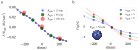
\includegraphics{figures/SPIE_results.png}}%%
    \caption{SPIE results.}
    \label{fig:SPIE}
\end{figure}

(CITE BENJAMINS WORK)

\subsection*{Strongly coupled optomechanical systems}

In strongly coupled optomechanical systems, the optical field can significantly modify the mechanical properties of the system, leading to a significant deformation
of the device, which in turn modifies the optical response. 

We have studied these systems in terms of topology optimization, as part of some unpublished work. In this work we consider 
the mechanical deformation of a membrane-like system, which is optically excited by a plane-wave. The optical field is calculated using the MST,
and the mechanical deformation is calculated using the linear elasticity theory. The mechanical deformation is then used to modify the optical field, 
leading to a self-consistent problem that can be solved iteratively, similar to other work.

ADD SOME OF THE WORK WITH THE MEMBRANE-LIKE SYSTEM HERE.


\section{Electro-optical systems~\cite{ownpub4}}

ADD PLOT FOR OPTIMIZATION RESULTS IN THE DIPOLE APPROXIMATION

Use Laser chaper in Hecht Optics book?

%\begin{figure}[tb]
%    \centering
%    \makebox[\textwidth][c]{\includegraphics{figures/electro_optic_review.png}}%%
%    \caption{Examples of electro-optical topology optimization. (a) Harmonic subtitute for transient topology-optimization of 
%    a heat conduction- convection problems, with applications in carrier diffusion systems; adapted from~\cite{carrier}. (b) Topology optimization of nanolasers 
%    accounting for diffusion of the gain media, adapted from~\cite{ownpub4}.}
%    \label{fig:opto_mech}
%\end{figure}


ADD WORKS ON TOPOLOGY OPTIMIZATION IN ELECTROSTATICS. POSSIBLY SOME WORK
ON COUPLED PROBLEMS? MEMS?

Talk about the laser cavity problem, and other works that include this effects.
Potentially add Rasmus's Schrödinger equation work.

electro-optical coupling refers to changing a device’s optical properties via an applied electric field (Pockels/Kerr effects). Pockels-effect (lithiumn niobate, galium arsenide), Kerr effect, electro-absorption effects (III-V) semiconductrs.
See also \url{https://en.wikipedia.org/wiki/Electro%E2%80%93optic_effect}

GIVE EXAMPLES OF COUPLED ELECTRO-OPTICAL SYSTEMS: imaging/sensing, telecommunications,
medical applications, optical interconnects, optical switches, optical modulators,
laser applications.

\subsection*{Topology optimization of nanolasers \cite{ownpub4}}

As an example of topology optimization in electro-optical systems in \cite{ownpub4} we study the design of nanolasers. 

\begin{figure}[tb]
    \centering
    \makebox[\textwidth][c]{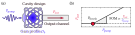
\includegraphics{figures/laser.png}}%%
    \caption{2d laser results.}
    \label{fig:laser3d}
\end{figure}



\begin{figure}[tb]
    \centering
    \makebox[\textwidth][c]{\includegraphics{figures/laser_2.png}}%%
    \caption{3d laser results.}
    \label{fig:laser3d}
\end{figure}
